\section{Methodology}
\label{sec:methodology}

\begin{figure*}[t]
\centering
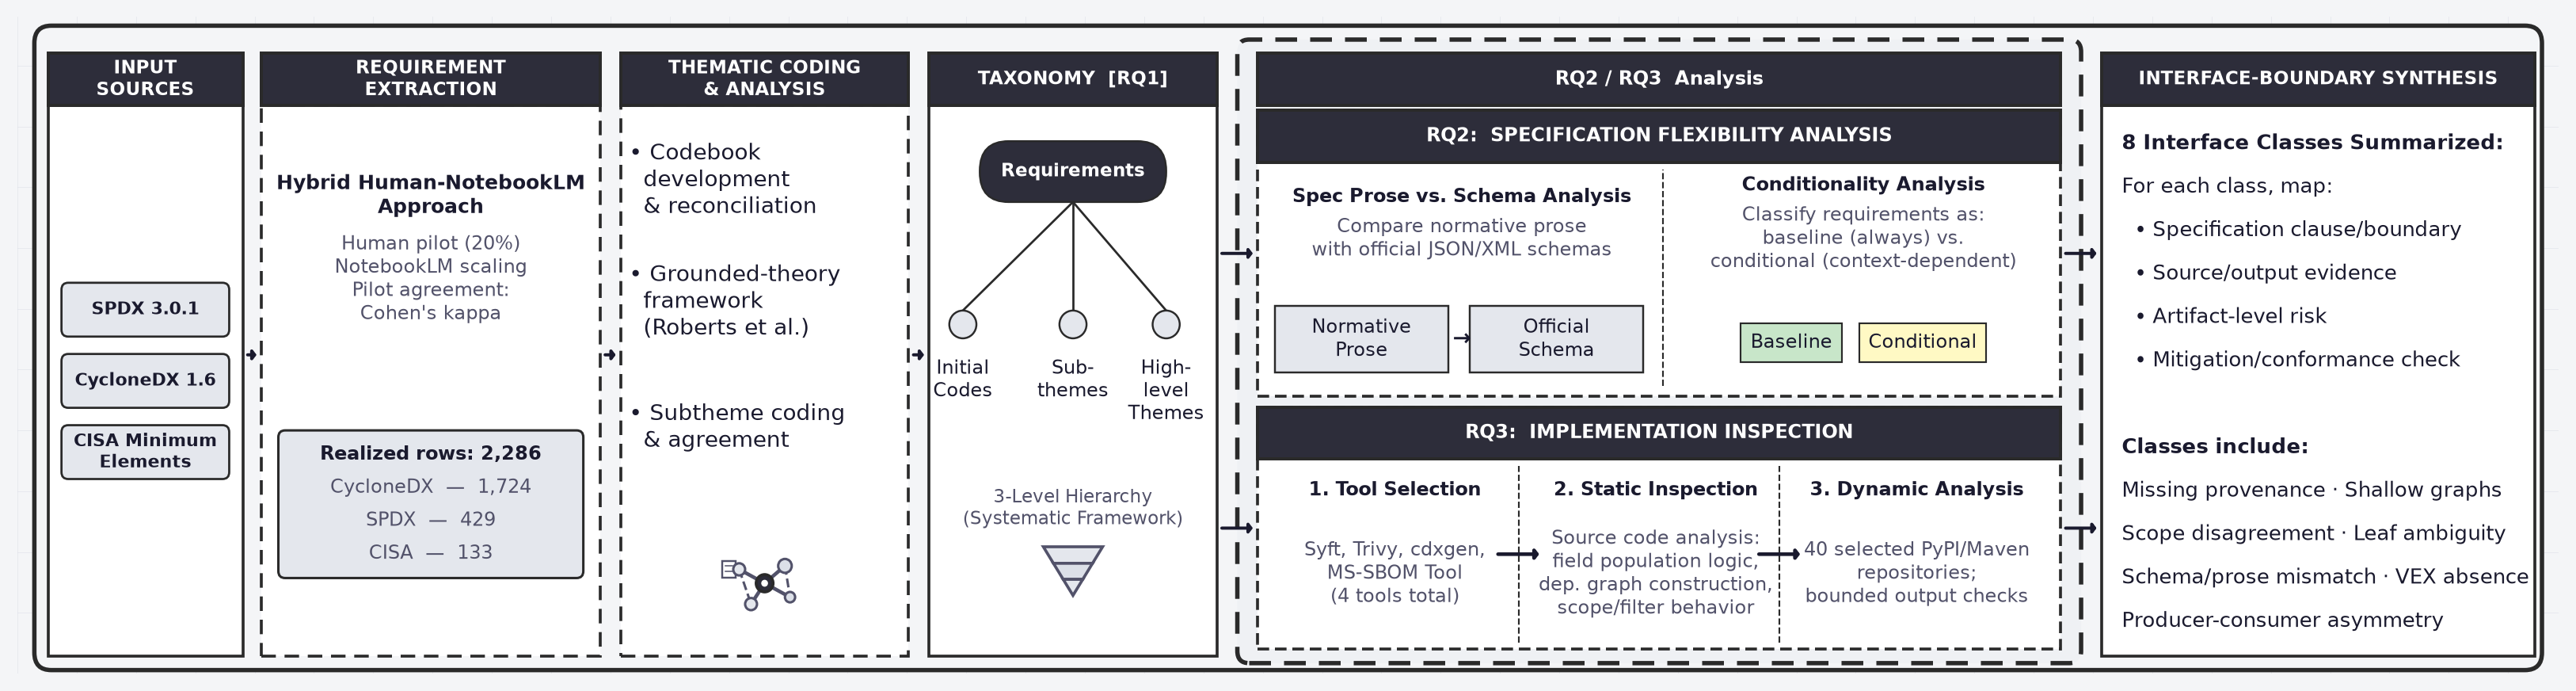
\includegraphics[width=\textwidth]{figures/methodology_pipeline.png}
\caption{Methodology pipeline; totals denote rows extracted under the stated protocol.}
\Description{Flowchart from three SBOM specification sources through requirement extraction, thematic coding, taxonomy construction, schema and conditionality analysis, four-tool implementation inspection, and synthesis into eight interface classes.}
\label{fig:req_analysis_pipeline}
\end{figure*}

Figure~\ref{fig:req_analysis_pipeline} connects specification text, generator implementations, and validation artifacts. RQ1 and RQ2 identify normative and structural boundaries; RQ3 traces selected boundaries through source and outputs.

\textbf{RQ1: What structural and semantic constraints do SBOM specifications impose on producers and consumers?}
We extract requirements from CycloneDX 1.6, SPDX 3.0.1, and CISA ME-SBOM. A requirement is a source statement or table unit constraining what a producer, consumer, document, or tool must, should, or may contain or do. Normative force follows RFC~2119-style \textit{MUST/REQUIRED}, \textit{SHOULD/RECOMMENDED}, and \textit{MAY/OPTIONAL} categories~\cite{rfc2119}.

\textbf{RQ2: To what extent do official schemas enforce the normative constraints defined in the specification prose, and where do they permit structural variation?}
We group requirements by purpose, compare normative prose with official schemas, and classify requirements activated only by optional classes, profiles, properties, or root objects.

\textbf{RQ3: How do generator tools implement the choices left open by specifications?}
We purposively inspect Syft and Trivy (both formats), cdxgen (CycloneDX), and Microsoft SBOM Tool (SPDX)~\cite{trivygithub,syftgithub,cdxgengithub,microsoftsbomtoolgithub}. All appear in prior empirical studies~\cite{reichmann2026poking,wangadherencegap2026}; the selection supports source-path comparison, not statistical sampling.

\subsection{Requirement Extraction}
We use a staged extraction process based on the grounded theory approach for analyzing technical guidelines \cite{chen2024}. A \emph{primary unit} is the smallest objective source segment evaluated for extraction: a complete sentence, list item, table row or cell, figure caption, or linked class/property definition. Annotators assign a binary decision to each unit, with 1 indicating that it contains at least one normative requirement and 0 indicating that it does not; a positive unit can yield multiple rows when it contains separable directives.

Two human annotators first applied this procedure independently to pilot samples covering 20\% of each specification, then reconciled disagreements. Cohen's Kappa in Table~\ref{tab:iar_kappa_scores} measures agreement on this binary extraction decision. We use $\kappa$ for the pilot because correctly agreeing to include requirement-bearing units and exclude non-normative units is part of establishing protocol reliability. Stage~1 agreement was lower for SPDX ($\kappa=0.458$) because its table-driven organization created boundary disagreements over whether a row, cell, or linked class definition constituted one primary unit. Because these disagreements included unitization, the Stage~1 score is a conservative consistency indicator rather than a strict chance-corrected estimate over a fixed unit set. After refining the unit-of-analysis and table-boundary rules, Stage~2 human agreement increased to $\kappa=0.820$ for SPDX, $0.827$ for CycloneDX, and $0.854$ for the CISA Minimum Elements for a Software Bill of Materials~\cite{cisaframing2024} (henceforth \textit{CISA ME-SBOM}).

The refined protocol was then scaled with Google's NotebookLM (accessed during July 2025). Human-to-NotebookLM agreement in Table~\ref{tab:iar_kappa_scores} uses the reconciled pilot material and measures the same binary primary-unit decision under the refined protocol.

After scaling, we conducted a held-out audit outside the 20\% pilot. For each specification, we randomly sampled 10\% of its pages from outside the pilot and divided them into the primary units defined above. Without viewing NotebookLM's output, the primary analyst independently applied the same binary extraction decision used in the pilot. Unlike the pilot's focus on protocol validation, this audit directly evaluates machine-extraction agreement on unseen source material using Cohen's Kappa. The resulting held-out agreement was $\kappa=0.922$ across 615 CycloneDX units and $\kappa=0.867$ across 52 CISA ME-SBOM units; the SPDX held-out score will be inserted after final verification. After scoring, a second analyst reviewed every disagreement with the primary analyst. This qualitative review found no major systematic omissions in the machine-extraction process and therefore did not alter the pre-reconciliation score.

The dataset contains 2,286 extracted rows: 1,724 from CycloneDX, 429 from SPDX, and 133 from CISA ME-SBOM. These totals describe the rows produced by the protocol, not a guaranteed exhaustive inventory. The CISA rows include directives about creation, exchange, lifecycle, framing, and data-field guidance, not 133 distinct minimum data fields.

Raw row counts are not directly comparable across specifications because specification structure affects the extraction unit. For example, CISA ME-SBOM expresses that a conformant tool needs to possess the mandatory data field ("Dependency Relationship"). The corresponding obligation is expressed in CycloneDX prose by the statement that a tool "should" populate the \texttt{dependencies} graph for every component, which we extract as one \texttt{SHOULD}-level row, and in SPDX as table rows describing the \texttt{Relationship} element and its permitted types. We use counts and percentages only for within-corpus description and audit navigation. Our clause-level conditionality, schema/prose, and implementation-trace arguments do not depend on the magnitude of the row totals.

Appendix~\ref{app:prompts} records the LLM extraction methodology and prompts used to scale the corpus. We retain the extraction files unchanged and treat them and the generated tables as auditable intermediate artifacts rather than reproducible ground truth. Exact regeneration is not guaranteed because NotebookLM is a closed, nondeterministic system. The final inventory and anonymous location of the supplementary archive remain marked in the artifact-availability statement.

\begin{table}[t]
\caption{Cohen's Kappa ($\kappa$) for Pilot Requirement-Extraction Agreement.}
\label{tab:iar_kappa_scores}
\centering
\resizebox{\columnwidth}{!}{%
\begin{tabular}{@{}llccc@{}}
\toprule
\textbf{Stage} & \textbf{Comparison} & \textbf{CycloneDX} & \textbf{CISA ME-SBOM} & \textbf{SPDX} \\
\midrule
Stage 1 & Human vs.\ Human & 0.732 & 0.779 & 0.458 \\
\midrule
\multirow{2}{*}{Stage 2}
    & Human vs.\ Human      & 0.827 & 0.854 & 0.82 \\
    & Human vs.\ NotebookLM & 0.782 & 0.815 & 0.75 \\
\bottomrule
\end{tabular}%
}
\par\smallskip
{\scriptsize\emph{Note:} The table reports pilot agreement; the post-scaling audit reports held-out kappa separately.}
\end{table}

\subsection{Thematic Coding}
\label{subsec:thematiccoding}

We interpreted the extracted requirements using a codebook-based thematic analysis following Roberts et al.~\cite{roberts2019attempting}:

\begin{enumerate}
\item \textbf{Codebook Development:} A primary analyst first coded a 20\% sample. During a sanity check, the analysts discussed ambiguous codes and category placement and agreed on consistent decision rules. The primary analyst then completed the full corpus, assigning each requirement to one subtheme, and formalized the resulting codebook with each subtheme's label and definition, inclusion/exclusion criteria, decision rules, and boundary examples. For example, \textit{Dependency Representation} includes requirements to record upstream/downstream component relationships and excludes component-identity requirements that name no relationship.
\item \textbf{Inter-Coder Agreement:} Using the finalized codebook, a secondary human annotator independently assigned one subtheme to each normative-requirement row in a stratified random sample targeting 25\% of each specification and spanning its sections. Agreement required an exact subtheme match with the primary analyst. Because each specification has a different subtheme codebook, we report within-specification exact percentage agreement rather than a pooled kappa. Pre-reconciliation agreement, calculated as $100\times A/(A+D)$~\cite{milesandhuberman1994,roberts2019attempting}, was 392/431 (91.0\%) for CycloneDX, 91/107 (85.0\%) for SPDX, and 28/34 (82.4\%) for CISA ME-SBOM. After recording these values, the annotators discussed every disagreement and assigned the final subtheme by consensus; reconciliation was not counted as initial agreement. This human-to-human thematic check is distinct from the requirement-extraction agreement in Table~\ref{tab:iar_kappa_scores}.

\end{enumerate}

After subtheme coding and reconciliation, semantically related subthemes were grouped into mutually exclusive high-level themes while retaining the underlying initial codes and subthemes; no subtheme was assigned to more than one high-level theme. For example, \texttt{dep\_graph\_population}, transitive-resolution, and dependency-scope codes form \textit{Dependency Representation} under \textit{Structural Completeness}. This labels structural-coverage requirements; it does not claim dependency ground truth.

For CycloneDX, the refined coding yields 13 merged subthemes and 7 final themes; for SPDX, 15 merged subthemes and 6 final themes; and for CISA ME-SBOM, 16 merged subthemes and 6 final themes. 

\subsection{Schema and Conditionality Analysis}
\label{subsec:schemaandconditionalityanalysis}
For schema analysis, we manually construct an expected schema based on the extracted normative requirements and compare it against the official machine-readable schemas. We classify mismatches into definition presence, property presence, property type, and requiredness/constraint differences. This comparison concerns machine-checkable structure; external dependency discovery, producer evidence coverage, and defensive-task sufficiency are evaluated through prose, profile, source, and output evidence rather than treated as JSON Schema obligations.

For conditionality, we construct a minimum template SBOM for each specification and map which requirements apply to that baseline. We then classify prerequisites for the remaining requirements, such as profile conformance, class instantiation, property presence, data type presence, serialization choice, or optional root-object inclusion. This measures the practical baseline enforced by the standard rather than the total size of the specification.

\subsection{Implementation Inspection}
\label{subsec:implementationinspection}
We combine manual source inspection with focused output validation. 

\textbf{Manual inspection.}
Fixed snapshots are Trivy v0.72.0, cdxgen v12.7.1, Syft v1.48.0, and Microsoft SBOM Tool v4.1.11; Table~\ref{tab:tool-evidence} records their exact commits, inspected formats, and source anchors. These snapshots define the evidence boundary and were re-verified in July 2026. They are not latest-release claims, and later versions would require reinspection. Following Chen et al.~\cite{chen2024}, we trace serialization entry points across provenance, component identity, dependency relationships, scope/filtering, and coverage/analysis signals. We record conditionality and surfaced omissions, requiring a repository-relative path for every source observation.

\textbf{Dynamic Generation.} To complement the static inspection, we conduct focused output validation across two package ecosystems: PyPI and Maven. For PyPI, we selected the top 20 packages by monthly download count, and for Maven, we selected the top 20 artifacts by reported usage rank, giving 40 selected packages in total \cite{pypistats, mvnrepository}. For each package we generated CycloneDX outputs with Syft, Trivy, and cdxgen, and SPDX outputs with Syft, Trivy, and the Microsoft SBOM Tool, aggregating one output per package per tool. This popularity-based set spans two ecosystems but is not statistically representative of
PyPI, Maven, or other ecosystems. We do not quantify inventory overlap, graph depth, reproducibility, or vulnerability-result variation; the artifacts provide bounded observations rather than frequency estimates or a comprehensive tool benchmark.

For the SPDX CISA-derived presence analysis, we operationalized ten valid checks: SBOM author, software producer, component name, software identifier, component hash, license, dependency relationship, tool name, timestamp, and generation context. We excluded a separate automated check labeled ``component version'' because it reads \field{CreationInfo.specVersion}, which records the document format version rather than a package's version. It is therefore a non-CISA document-format control and appears in neither the numerator nor denominator reported in Section~\ref{subsec:cisa-compliance}.

Our specification analysis (Section~\ref{sec:spec-analysis}) targets SPDX 3.0.1, but Trivy and Syft produce SPDX 2.3 natively. Their generation behavior therefore originates under SPDX 2.3, not under SPDX 3.0.1. We converted their native artifacts to SPDX 3.0.1 using the official SPDX Online Tools converter \cite{spdxonlinetools}, which wraps the SPDX Workgroup's reference Spdx2to3Converter, solely to obtain a common representation baseline. Conversion between major versions is a defined field-and-type mapping rather than a lossless transform, and prior work reports that conversion can reinterpret or drop fields \cite{sbomlandscape}; we do not infer that these tools' historical implementation choices were caused by SPDX 3.0.1.

\textbf{Conversion Fidelity Check}. For reported cross-version field-presence comparisons, we locate the corresponding field in the native 2.3 artifact and confirm whether its presence or absence remains visible after conversion. Any native/converted discrepancy is attributed to conversion and excluded from generator-level findings. This check supports representational comparability; it does not establish causal traceability from a 3.0.1 clause to a tool implemented for 2.3.

\subsection{Synthesis Output}
The evidence-chain synthesis links each boundary to its specification source, implementation/output observation, artifact-level risk, and mitigation without assigning a single cause.
